\documentclass[10pt, letterpaper, oneside]{article}

\usepackage{graphicx}
\usepackage{epsfig}
\usepackage{verbatim}

\pagestyle{headings}

\author{Conor McGann}

\title{The EUROPA Solver Framework}

\begin{document}

\maketitle

This document outlines the requirements and technical approach for controlling the search undertaken by the standard EUROPA solver. We assume a chronological-backtracking, heuristically guided, refinement search.

\section{Preliminaries}
In our planning paradigm, a solver is a problem solving actor which operates to resolve flaws in a plan database. Informally, a flaw is an indication of a potential for inconsistency in a given partial plan. We distinguish 3 types of flaw, each with its own corresponding  procedure to resolve it:
\begin{enumerate}
\item An Object Flaw - arises when an ordering is required for tokens associated with an object. This occurs in objects such as {\em Timelines} to ensure that a mutual exclusion is enforced, and on metric resources to ensure that the resource level is within specified limits.
\item A Token Flaw - arises when a token is in the {\em Plan Database} but not yet in the {\em Plan}. Such a token is said to be {\em inactive}. Token Flaws are resolved through merging with an existing token already in the plan, through insertion as a new token in the plan, or through rejection, if permitted.
\item A Variable Flaw - arises if there are variables of tokens already in the plan whose values have not been specified. Such a variable is said to be {\em unbound}. Variable Flaws are addressed by specifying a value for the domain. 
\end{enumerate}

Within the standard search procedure we distinguish 3 elements of search control which provide the tools for tuning and customization to particular applications and domains:
\begin{enumerate}
\item Scope Definition - defines the set of flaws that must be resolved to complete the plan. When there are no flaws remaining, and the plan database is not inconsistent, the plan is considered complete and the solver terminates.
\item Flaw Selection - identifies which flaw to resolve next.
\item Flaw Resolution - executes appropriate underlying procedures to resolve a flaw, until all stipulated options are exhausted. These underlying procedures include the actions already mentioned e.g. token activation, token merging, token ordering, variable binding. In addition they must address aggregation and ordering of choices for resolution. Note that a flaw may persist after resolution steps have been taken. For example, a {\em Timeline} may require additional orderings in order to ensure the temporal mutual exclusion is satisfied.
\end{enumerate}

The focus of this document is to provide the means to efficiently, compactly and flexibly customize each of the above elements of search control to provide a versatile solver.

\section{Requirements}
This section reviews by example the main components of search control and presents observations for generalization of the requirement or to consider as we further develop the technical approach.
\subsection{Scope Definition}
In general, there may be many sophisticated ways in which the scope of flaws for a solver to work on can be specified. We look at this from the point of view of filters applied to the built in set of system flaws described earlier. Examples of the criteria that have arisen include:
\begin{enumerate}
\item Exclude all singleton {\em Variable Flaws} that are not guards in a rule.
\item Exclude all token flaws whose timepoints are not necessarily contained by the solvers horizon. This is a dynamic flaw filter in that it may have to be re-evaluated if the timepoints are restricted.
\item Exclude all temporal variable flaws. This is a static flaw filter since a variable is always a temporal variable.
\item Exclude all variable flaws with the name {\em foo}. This is a static flaw filter since the name of a variable cannot change.
\item Exclude all variable flaws with infinite domains. This may be a static filter for some variables and a dynamic filter for others. For example, all variabes with enumerated domains are finite. Interval domains may be finite if they are singletons, or if they are restricted to integer values and have finite bounds.
\item Exclude all variable flaws with the name {\em foo} unless they are singletons. This is a dynamic filter since it must be re-evaluated as the domain is restricted.
\item Exclude all object flaws on objects of class {\em Foo}. This applies to all subclasses of {\em Foo} also.
\item Exclude all variable flaws on all tokens of all objects of class {\em Foo}. This is a static filter.
\item Exclude all token flaws which can be rejected until there are no token flaws which cannot be rejected. This is a dynamic filter that should be re-evaluated as tokens change their state or are added to the plan database.
\item Exclude all start variables of all tokens of predicate {\em Bar} unless the start variable is a singleton or the level of the resource between the lower bound of the start variable, and a horizon {\em h} exceeds a given threshold. This is a dynamic filter.
\end{enumerate}

\subsubsection{Observations}
We consider that the requirements of scope specification can be considered in 2 parts:
\begin{enumerate}
\item What filters should be considered for a given object, token or variable flaw? This is a problem of matching the scope specification of a filter with the context of a flaw. Note that multiple filters may apply.
\item What test should be applied once the filter is obtained? In the simplest cases, this is trivial, since the match against a scope specification is sufficient to conclusively exclude a flaw. For example, filtering all temporal variables by filtering on the names of start, end and duration will easily exlude any Variable Flaws with these names. However, it may be more complex requiring arbitrary procedures to be executed to evaluate rich and possibly only remotely connected contextual information. This scenario was illustrated where a Flaws is filtered babsed on a resource level over an interval of time.
\end{enumerate}

\subsection{Flaw Selection}
There are many conceivable ways in which the next flaw to work on can be determined. Here are some examples:
\begin{enumerate}
\item Prefer unit variable flaws over all other flaws. The rationale behind this approach is based on the combination of prefering the most constrained flaw with the cheapest cost to find such a flaw.
\item Prefer unit token flaws over all other flaws except unit variable flaws.
\item Prefer non-variable flaws participating in a conditional subgoal over non-unit variable flaws not participating in a subgoal.
\item Prefer Object Flaws with the least number of ordering choices.
\item Prefer token flaws most recently created. The rationale for this approach is to recognize that many goals in a plan may be quite independent of one another. 
\end{enumerate}

\subsubsection{Observations}
One has to carefully consider the cost of computing sophisticated heuristics with their benefits. One should like to experiment with these matters as a planning problem is being tackled and the nature of the search is becoming apparent. Stronger heuristics may need to be introduced in a targetted fashion to address particularly troublesome aspects of the search. In contrast, cheap and naive methods may well suffice where choices seem to have little impact on the problem. Thus we have a few key points:
\begin{enumerate}
\item We must be able to customize the heuristic evaluation technique for targetted subsets of the set of flaws.
\item Given that we will likely end up in a division of the set of flaws into subsets governed by specialized techniques, it is imperitive to have a globally agreed priority scheme to allow one group to over-ride another, and also to permit a cut-off prior to visiting all flaws if a current best priority cannot be beaten.
\item It must be possible to unambiguously relate a flaw to exactly one flaw selection mechanism. This relationship can be static or dynamic.
\end{enumerate}

\subsection{Flaw Resolution}
Once again there is quite a spectrum of complexity for resolving flaws. Here are some examples encountered so far:
\begin{enumerate}
\item Prefer values in ascending order of all Variables of all Tokens on all objects of class {\em Foo} or its subclasses.
\item Prefer values in descending order for all Variables of the name {\em foo}
\item Randomly select from all possible values for all Variables on all Tokens of all objects of class {\em Bing} using a uniform distribution.
\item Prefer merging with tokens with minimal {\em distance} from the inactive token. This selects the least constraining value in some sense.
\item Select a single value for all variables with name {\em foo} by request from external agent {\em WeatherSensor}.
\item Prefer to place tokens as early as possible for all instances of the class {\em Bar}.
\item Prefer values on variables of tokens of predicate {\em Baz} which have the highest value for the function {\em func}.
\item Prefer resolving token flaws through merging over activation. This is based on the intuition that merging will produce a smaller plan.
\end{enumerate}

\subsubsection{Observations}
There is clearly a diversity of resolution schemes. Once again we see the need for a targetted approach allowing very specific and quite esoteric methods to be used and also for very straightforward methods to be used. The former are most likely relevant for key parts of the search, for whatever the purposes of the solver. We note the following additional points:
\begin{enumerate}
\item We must be able to customize the flaw resoultion technique for arbitrary subsets of the flaws.
\item It seems highly desireable to seek a close collaboration between Flaw Selection and Flaw Resolution since the data obtained to select the next flaw to work with, which may have been costly to obtain, is more often than not going to be directly useful to the Flaw Resolution technique. For example, computing the set of tokens with which a given token can be ordered is often useful to determine its priority as a flaw and is immediately useful as input to the resolver. 
\item It may be desireable to scope Flaw Resolution mechanisms within the scope of Flaws of a given Flaw Selector.
\end{enumerate}


\section{Technical Approach}
In this section we make the case for a dynamic plug-in approach for customization of the solver. To ground that we present the core planning algorithm and indicate where components can be plugged in. We go on to describe a proposed syntax and semantics for matchable expressions which can be used for configration control, and describe the interfaces which will be provided to integrate search control components. Finally, a set of standard components are described and examples of how they can be configured for a solver will be presented.

\subsection{Most Basic Design Decision}
There are 2 basic approaches to accomplishing the search control capabilities described. The first is to develop a rich and expressive scripting language which can be used to address each area of Scope Management, Flaw Selection, and Flaw Resolution in a context dependent manner. The second is to prefer a hybrid approach which uses a combination of a specialized language as a means to bind to specialized C++ code for final computation in each case. This second approach focuses on fast matching of entities based on local contextual information for each flaw type, and binding to pre-compiled plug-ins. The former approach has the advantage that it will most likely result in a coherent language for describing a carefully circumscribed set of search control capabilities. Its principal disadvantage is that it will likely be:
\begin{enumerate}
\item complex as it attempts to cover a broad scope of scenarios
\item inevitably deficient and hence limiting
\item costly to develop and maintain
\end{enumerate}

The latter, hybrid approach offers flexibility and extendibility since we can plug in arbitrary procedural code to address the requirements of {\em flaw selection} and {\em resolution}. It will lead to more efficient sytems since specialized, optimized code can be inserted for particularly costly calculations. It will also be less costly to develop and maintain since it permits rapid development of basic functionality and targetted incremental development of additional capabilities. The main disadvantage of the hybrid approach is that of reduced transparency for a user since the semantics of final calculation will be specific to component plug-ins. This is similar to the drawback of using procedural constraints instead of specifying the semantics of a constraint explicitly in the language. Arguably, there is a further potential draw-back in that there may be more of a requirement on the part of the application developer to have recourse to C++ programing. This can be augmented with a reasonable set of available plug-ins, which will be enhanced over time. We shall proceed with the hybrid approach.

\subsection{The Chronological Backtracking Planning Algorithm}
The structure of the planning algorithm provides us the template which we instantiate to provide a specific solver. The general planning algorithm is outlined below. Note that the algorithm takes as input an initial {\em Plan Database} containing a partial plan, and a set of {\em Flaw Managers}. A {\em Flaw Manager} will be responsible for obtaining the set of {\em Flaws} within some confined subset of overall {\em Flaws}. A {\em Flaw Manager} is further resposnible for formulating a {\em DecisionPoint} to address a {\em Flaw} under it's control. A {\em Decision Point} encapsulates the details of what operations on the partial plan can be taken and in what order they should be tried.
\begin{verbatim}
Result plan(PlanDatabase db, FlawManagers fms){
  if(!checkConsistency(db))
    return INITIALLY_INCONSISTENT;

  // Initialize the stack for closed decisions
  Stack s = {};

  // Allocate the next decision point, if
  // there is one. Incorporates the services of
  // Scope Management and Flaw Selection
  DecisionPoint dp = 
   selectDecisionPoint(db, fms);

  while(dp != NULL){
    // Exhaustively try current decision point.
    // Incorportaes the services of Flaw Resolution
    while(dp.hasNext()){
      dp.tryNext();
      if(!checkConsistency(db))
        dp.undo();
    }

    // If not consistent, have to undo last
    // closed decision
    if(!checkConsistency(db)){ // Exhausted choices
      if(s.isEmpty())
        return SEARCH_EXHAUSTED;
      else {
        dp = s.pop();
        dp.undo();
      }
    }
    else {
      s.push(dp);
      dp = selectDecisionPoint(db, fm);
    }
  }

  return PLAN_FOUND;
}
\end{verbatim}

The function {\em selectNextDecisionPoint} is listed below. It takes a {\em Plan Database} and a sequence of {\em Flaw Managers}. Note that the algorithm evaluates all {\em Flaw Managers} in order until it finds a {\em Decision Point} with the best heuristic score (i.e. lowest priority value). A {\em threshold} is used to permit a cut-off as soon as a decision point is discovered which we know to be a best choice. This value is 1, recognizing that as soon as a unit decision is discovered, or a point of no choices available, we can exit immediately. The ordering of flaw managers is important in that it defines the ordering if all other things are equal.
\begin{verbatim}
DecisionPoint selectDecisionPoint(
                      PlanDatabase db, 
                      FlawManagers fms){
  unsigned int priority = WORST_PRIORITY;
  FlawManager fm = getNextFlawManager(db, fms);
  DecisionPoint bestDecision = NULL;

  while(priority > BEST_PRIORITY && fm != NULL){
    DecisionPoint candidate = 
     fm.getNextDecisionPoint(db, priority);

    if(candidate == NULL)
      fm = getNextFlawManager(db, fms);
    else
      bestDecision = candidate;
  }
  return bestDecision;
}
\end{verbatim}

In summary, observe the following points of flexibility for controlling search according to the above scheme:
\begin{enumerate}
\item A sequence of {\em Flaw Managers} can be passed to the planning algorithm to configure its scope. These components will be visited in the order defined in the sequence on input.
\item The algorithm to obtain the next decision point is encapsualted for each {\em Flaw Manager}. This is according to their respective implementations of {\em FlawManager::getNextDecisionPoint(PlanDatabase db, unsigned int priorityToBeat)}.
\item Algorithms and data structures to formulate the ordered set of choices for resolving a flaw, and the execution of a choice, are completely encapsulated within the {\em DecsionPoint} class, which is allocated by the responsible {\em Flaw Manager}.
\end{enumerate}

\subsection{The Search Control Object Model}

\begin{figure*}[t]
\includegraphics[scale=0.75]{SearchControl.eps}
\caption{Search Control Object Model}
\label{SearchControlFramework}
\end{figure*}

Figure \ref{SearchControlFramework} is a UML class diagram of main elements of the {\em Search Control Object Model}. The core collaboration is between the following elements:
\begin{enumerate}
\item Solver - provides the core algorithm and data structures to accomplish a chronological backtracking heuristic search. It deals in abstract constructs of {\em Flaw Managers} and {\em Decision Points}. These abstractions allow the planner to delegate responsibility for how to manage scope, flaw selection, and flaw resolution to components that may be plugged in. Thus we use the planner as an example of a {\em Template Pattern} for providing configurable search control.
\item FlawManager - provides for the flaw selection from a given subset of flaws defined to be in scope. It uses a pair of {\em Flaw Filters} to manage static and dynamic scoping rules. The system shall ensure that Flaw Managers manage disjoint sets of {\em Flaws}.
\item FlawFilter - the only responsibility of this class is to answer the question: is a given flaw in scope? In contrast to previous designs, this class {\em does not} maintain the set of all flaws. This prevented combining a flaw selection heuristic with a test for scope. Such a combination may exploit opportunities for early termination when a flaw of highest priority (such as a unit decision) is found. Experience shows that such flaws are common. Each {\em FlawManager} is constructed with a {\em StaticFilter} and a {\em DynamicFilter}. 
\item StaticFilter - separates out scoping criteria that always return the same answer for any candidate flaw. 
\item DynamicFilter - may be re-evaluated a number of times before a candidate flaw actually comes into scope. For example, we may wish to filter a guard variable until it becomes a singleton. A {\em DynamicFilter} should have the property that once it permits a flaw to be in scope, it will remain in scope for all subsequent restrictions of the partial plan until it is resolved. Such an assumption, which seems quite reasonable in practice, permits internal caching which will be advantageous. In addition, the {\em DynamicFilter} enforces a given horizon as a built in behavior. Finally, the {\em DynamicFilter} uses a set of {\em FilterConditions} to allow flexible customization through {\em plug-ins}.
\item FilterCondition - implements a specific test for a candidate flaw. A candidate flaw must pass all {\em relevant} filter conditions to be included in the scope.
\item DecsionPoint - provides the means to formulate the set of choices and visit those choices in a priority order. The interface allows us to encapsulate all the details of how to store candidate choices, how to order them, and how to track what has been tried already. Note that there is an opportnity for close collaboration between a particular {\em FlawManager} and a particular {\em DecisionPoint} since the details of allocation are encapsualted within implementation components rather than at the core interface level. This removes a potential performance problem. For example, in order to decide which Object Flaw to work on, the {\em ObjectFlawManager} will likely be determining the set of possible ordering choices for a given token. Computing this set can be expensive, and so it makes sense to permit the information to be directly exploted by an {\em ObjectDecisionPoint}. With this approach, these trade-offs can be freely explored based on performance profiling and optimized as needed.
\end{enumerate}

Strictly speaking, subclasses of {\em DecisionPoint} and {\em FlawManager} are not part of the core object model. This is because an implementation could be provided which did not use them, but rather preferred for example to have a single {\em FlawManager} and a totally different rationale for specializing {\em DecisionPoint}. However, there is a string motive for separating out management of token, object and variable flaws, since the events that need to be tracked and the logic for tracking them is quite different for each such case. Similarly, the structure of decisions for object, token and variable flaws is very different. Therefore, we will develop our componenet structure using this further separation of concerns according to flaw type.

\subsection{Configuration}

\begin{figure*}[t]
\includegraphics[scale=0.75]{ConfigurationFramework.eps}
\caption{Plug-in Configuration Framework}
\label{ConfigurationFramework}
\end{figure*}

The previous section outlined the {\em Search Control Object Model}. We can customize any given planner by plugging in specializations of:
\begin{enumerate}
\item {\em FlawManager} or its descendants.
\item {\em FlawFilter} or its descendants.
\item {\em FilterCondition} or its descendants.
\item {\em DecisionPoint} or its descendants.
\end{enumerate}
We can also customize a given planner by allowing for different data to be used to configure a given component. For example, a {\em StaticFilter} is not likely to be subclassed unless a new expression capability is to be added which cannot be added to the base class (for whatever reasons). Therefore, we would wish to customize a static filter component through the set of expressions we want to use to match flaws to be excluded from the planner's scope. A {\em StaticFilter} might be thought of as a {\em heavy component} since it is heavily data driven to specialize its behavior, rather than subclassed. In contrast, we can imagine creating an extension to a {\em VariableDecisionPoint} to achieve a Min order vs. a Max order. Such an extension would have no configuration data to customize it further, and might be consdidered a {\em light component} since it provides no data driven range of behaviors. To illustrate this further, the design described here could be evolved to be based on only a few components and an elaborate scripting language passed in to configure its behavior. The reason we desire this range is to support an evolution of the implementation as we are able to develop more sophisticated components to provide a more coherent and usable system to end-users. This will limit possibilities of users blocking on a centralized implementation as they can freely plug-in relatively small specializations at the fringes of the design. To accomplish this, we require a component configuration framework that can link planning entities to concrete component implementations, and pass in data to those implementations as needed. The scheme for doing this relies on an {\em Abstract Factory} design pattern an is illustrated in Figure \ref{ConfigurationFramework}.

\subsection{Application Developers Perspective}
In this section we outline the design from the perspective of the application developer i.e. user seeking to solve a planning probblem with EUROPA.

\subsubsection{The basic configuration file structure}
An aplication developer will create an xml file to configure the planner. For this first simple example, suppose we want a planner to only make variable binding decisions, to exclude making any bindings on temporal variables, and variables of infinite or dynamic domains. This is a common requirement. Further assume that in general we want to pick the least value first, but in the case of setting the value for the speed of a drive token, we want to prefer to try choices in descending order. Finally, in the particular case of selecting values for {\em wind speed} variables fin {\em data} tokens on {\em Weather} object types, we wish to use a random selection with a uniform distribution and a cut-off which indicates how many of the possible values we want to try before admitting defeat. The XML snippet below illustrates how this might look.
\begin{verbatim}
<planner name=''MySamplePlanner''>
 <flaw-manager component=''VariableFlawManager''>
   <static-filter component=''StaticFilter''>
     <expression scope=''*.*.start''/>
     <expression scope=''*.*.end''/>
     <expression scope=''*.*.duration''/>
   </static-filter>
   <dynamic-filter component=''DynamicFilter''>
     <expression scope=''*.*.*'' 
                 component=''InfiniteOrDynamic''/>
   </dynamic-filter>
   <resolver scope=''*.*.*'' 
             component=''MinValue''/>
   <resolver scope=''*.Drive.speed''
             component=''MaxValue''/>
   <resolver scope=''Weather.data.windpseed''
             component=''RandomValue''>
     <data name=''distribution'' value=''Uniform''/>
     <data name=''cutoff'' value=''3''/>
   </resolver-scope>
 </flaw-manager>
</planner>
\end{verbatim}

The key things to note are:
\begin{enumerate}
\item A nested structure for components. The planner will be passed the XML element which in this case is the root. The planner will iterate through the child nodes. Components names of {\em VariableManager, StaticFilter, DynamicFilter, InfiniteOrDynamic, MinValue, MaxValue, and RandomValue} will be used to obtain a concrete factory. Such factories will be passed in the xml element, which will include child nodes. The allowable data in the child nodes can be completely customized to each component.
\item In this example, the planner is configured with only one {\em Flaw Manager}. This planner is thus only capable of making variable binding decisions. It will not address any {\em Object Flaws} of {\em Token Flaws}. No limit is placed on the number of {\em Flaw Managers} that may be configured.
\item The order of definition of a {\em Flaw Manager} is the order in which they will be visited in the implementation of the function {\em selectNextDecisionPoint}.
\item A {\em Resolver} binds to an instance of a {\em DecisionPoint} class. In the above example, resolvers are used for ordering and pruning. Such a role leaves the opportunity for incomplete search at the discretion of the application developer. Such details are encapsulated within a component.
\end{enumerate}

\subsubsection{Component Registration}
The configuration model outlined requires registration of concrete factories in the main application, or elsewhere, to link logical component names with actual C++ classes. A macro will be provided to make this quite straightforward. A fragment of C++ code to register required components is provided below:

\begin{verbatim}
REGSITER_COMPONENT(``VariableFlawManager'', 
                   EUROPA::VariableFlawManager);
REGSITER_COMPONENT(``StaticFilter'', 
                   EUROPA::EUROPA::StaticFilter);
REGSITER_COMPONENT(``DynamicFilter'', 
                   EUROPA::DynamicFilter);
REGSITER_COMPONENT(``InfiniteOrDynamic'', 
                   EUROPA::InfiniteOrDynamicFilterCondition);
REGSITER_COMPONENT(``MinValue'', 
                   EUROPA::MinValueHeuristic);
REGSITER_COMPONENT(``MaxValue'', 
                   EUROPA::MaxValueHeuristic);
REGSITER_COMPONENT(``RandomValue'', 
                   EUROPA::MonteCarloSelector);
\end{verbatim}

\subsection{Possible elaborations for Expressions}
As already mentioned, our design uses a simple but powerful matching mechanism to provide links between Flaws and their relevant filters, and heuristics. We can expand this capability over time to use a richer language for defining such matching expressions. This section outlines the kind of language we would propose, based on an existing verification language we developed for the purposes of regression testing.

\subsubsection{The local context for expression evaluation}
We are focussed on matching against the local context of Objects, Tokens, and Variables. The approach for doing this is based on the relations between these entities arising in the schema and the plan database. The relations of interest are:
\begin{enumerate}
\item isA(ObjectType, ObjectType) - defines an inheritance relation between object types (STATIC).
\item isA(objectName, ObjectType) - defines an object name in the plan database to be of a certain type (STATIC).
\item hasA(ObjectType, ObjectType, ObjectName) - defines a composition relation between object types (STATIC).
\item hasA(ObjectType, Variable Type, Variable Name) - defines a composition relation where variables are composed in Objects. In current implemenations, such variables will not be flaws as they are required to be singleton values on construction. We include it here for completeness (STATIC). 
\item hasA(ObjectType, Predicate) - defines a 1 to many relation associating a given predicate with all instances of a given object type (STATIC).
\item hasA(Predicate, Variable Type, Variable Name) - defines a 1 to many relation associating a set of variables with a Predicate (STATIC). Note that this includes local variables introduced in rules.
\item hasSubGoal(Token, Token, TemporalRelation) - defines a relation between a master token, and its subgoal, with a qualification for the nature of the TemporalRelation (i.e. any, meets, metby, starts, ends....). This relation is dynamic since a given relation may not exist immediately but may be added as additional subgoal rules are triggered.
\item hasDomain(Variable, Domain) - relates a set of domain values to a variable. This is a DYNAMIC relation since the set of values change as planning progresses. Note that certain expressions may take advantage of the monotonic restriction of the set of values to avoid re-evaluation of expressions over domains.
\end{enumerate}

\subsubsection{Outline for language sytax and semantics}
In general, the syntax for expressions follows that developed for validating that certain patterns exist in partial plans using the {\em Aver} test language. This syntax is based on functions for returning sets of obects, tokens and variables: Objects(query-spec), Tokens(query-spec) and Variables(query-spec), were:
\begin{enumerate}
\item query-spec takes the form: [operand operator operand [ AND operand operator operand [..] ]]
\item all operands resolve to a domain of values
\item an operand can be a multi-valued literal domain such as {'A' 'B' 'C'} or [0.4 100.23]
\item an operand can be a singleton value literal such as 'A' or 7.82 or 'fooObjectName'
\item an operand can be derived from the properties of a local context e.g. this, objectType, predicateType, varType,  start, end, duration, state, object, userDefinedVariableName, domain. Note that the set of such properties is entirely dependent on the entity context in which they are being resolved.
\item an operand can be a function on an operand: operand-function(operand). Examples of operand functions include: min, max, temporal-relations, ancestors, singleton
\item an operator is drawn from the set of basic domain operations: {\em $>, <, <=, >=, ==, !=$, in, out, intersects}.
\end{enumerate}

Here are some sample expressions using this scheme:
\begin{enumerate}
\item ``Variables(objectType in \{'Foo' 'Bar' 'Baz'\} AND singleton(domain) == false)''. This will match all non-singleton variables on all tokens on all objects whose object type is in the given set.
\item ``Tokens('Timeline' in ancestors(objectType))''. This will match all Tokens on all objects whose object type is derived from a Timeline.
\item ``Tokens(object == 'navigator' AND speed in [3 7])''. This will match all tokens whose object variable is a singleton value with the name 'navigator' and the speed predicate variable is in the range [3 7].
\end{enumerate}

\subsubsection{Evolution and Intergration}
Most of the component framework presented can be used independently of the matching engine, which is used by the {\em FlawManager} and {\em FlawFilter} classes. We would be starting out with a very simple matching engine as noted. However, we can easily pre-process more simplistic expressions into the new sytax. For example, {\em ``*.Drive.speed''} becomes {\em ``Variables(predicate == `'Drive' AND name=='speed'''}. In the interim, we can create components for dynamic filtering and static filtering on an as needed basis that implement specific restrictions not available with the base expression capabilities. For example, the folowing might be used to filter out all variable binding decisions on drive tokens which may still be rejected.
\begin{verbatim}
  <dynamic-filter scope=''Rover.Drive.*'' 
                  component=''PQLExpression''>
    <intersects variable=''state'' 
                value=''{'Rejected'}''/>
  </dynamic-filter>
\end{verbatim}

In the above example, we assume the existence of a standard component for evaluating expressions of a plan query language.

\section{Notes on ObjectFlaws}
An Object Flaw arises where additional ordering constraints are required upon the tokens associated with that object. In EUROPA 1 and in the CBPlanner, a Token-centric perspective was taken i.e. one considers a token to inherently require some ordering on an object. The flaw model would then compute the aggregate set of ordering choices over all possible objects. In EUROPA 1 this wold retrieve all slots across all timelines. In EUROPA 2, this obtains all ordering pairs across all objects. There are 2 issues with this approach:
\begin{enumerate}
\item It is costly in general to construct such a large set of token ordering choices, since one must potentially evaluate many options and the cost for evalutaion of an option is relatively high.
\item It seems un-intutitive in the general case of tokens and objects to raise the flaw from the token's perspective. Flaw detection should be based on the object which is the source of the issue. For example, one a timeline, all tokens must be totally ordered. If active tokens on a timeline could overlap then we should require additional ordering decisions. Similarly for a metric resource. If an envelope could be violated, but might not be, then we are concerned to reduce the flexibililty of tokens on that resource such that they bring the limits within bounds sufficiciently. An object is in a position to know this most effectively.
\end{enumerate}

If we take an Object perspective, then under current circumstances, an Object which has tokens to order will raise flaws for each such token, and the choices will be developed once the token is selected. Currently, a token may be considered for ordering even though its object variable has not yet been bound. This means that we cannot conclude a dead-end simply becuase there are no viable ordering choices for this token on this particular object. This is because it could be removed from the object as an acceptable strategy since it need not be placed on that object. This is arguably a good approach since it permits an incremental resolution of the actual flaw, and does so in a way that is information rich - the relevant tokens and constraints on that object are localized with the decision to order or exclude it. In contrast, we could require that flaws are only raised when a token is necessarily placed on an object (i.e. its object variable is a singleton). This would be quite simple and have the advantage that the decision model for resolving object flaws remains limited to simply posting token ordering constraints. However, we would lose some ability to work on the object flaws earlier in the planning process, and it would change the search structure. Furthermore,  it makes it very difficult to structure a search preference for ordering a token prefering particular locations across different objectcs before other locations. If we view it from a single object perspective, then that information is not readily available in the context of decision making, and one is forced to commit to an object before committing to a temporal position in the plan.

This then begs the question of finding the best way to maintain the total set of tokens to order, since these are the TokenOrder flaws. Trivially we can assume that all tokens, once activated, require an ordering. However, this is problematic since that token may require more than one ordering in the case of a metric resource, or it may not require any ordering at all if there is no overlap possible for this token. What we would really like is that the set of tokens that actually require orderings is propagated by the objects (i.e. resources in general). Alternatley, we might not propagate it, but rather just poll for it. It would be nice to defer that decision but build in the api.

A further issue with respect to flaw filtering on objects. The concept would be to ignore ordering requirements induced by certain objects. However, if we view the situation from the perspective of tokens, then we may formulate resolutions for a token with constrain it to an oject that has been filtered out. Should we allow this? To prevent it we would have to sacrifice completeness. The view for now is that we would only filter the generation of the flaw, but not prevent the resolution of the flaw from including choices on an object that would otherwise be filtered. In order to exclude choices, it seems like we have to think in terms of access control rather than flaw filtering.

Yet another issue - the way we structure choices around a token is just wrong in the case of resources in general. It imposes a decision for each token, and can thus impose a dependency in the solution on which decision you select to work on. This is not a problem with a timeline since every token requires and ordering. However, in a resource, things are different and we do not want to require an ordering but yet one of the nXn orderings (or more) may be required in order to solve the resource flaw. This can be alleviated by the NO-OP of constraining a token with respect to itself. In a timeline this covers the special case of an insertion in an empty timeline. However, that is only required since we base the flaw on a token being active, and thus requiring such insertion. Rather, we should not have to make such a commitment, but it is a small matter. So, to recap, resolution of this issue is accomplished by permiting a choice that can effectively be a NO-OP for a resource. The api already permits this and the response will be dependent on the underlying concrete class - Timeline vs Resource.
 
\section{Conclusion}
The proposed system can be functional in a matter of a few weeks. From there we can develop the capabilities in an incremental fashion. Future work may look at variations of the core planning algorithm to explore alternate search strategies. For example, incorportaing backjumping. However, given the flexibility provided, we expect that a large class of search engines can be assembled based on the simple chronological backtracking planner outlined.
\section{Gloassary}
\begin{enumerate}
\item Flaw
\item Metric Resource
\item Object
\item Partial Plan
\item Plan
\item Plan Database
\item Planner
\item Timeline
\item Token
\item Variable
\end{enumerate}
\end{document}j